\section{Introduction}

In this chapter I describe the design and implementation of OmniTune,
an extensible, dynamic autotuner, capable of runtime prediction of
optimisation parameters using machine learning. First, I describe the
architecture and public interface exposed by OmniTune, demonstrating
the communication pattern between the autotuner and SkelCL
applications. This is followed by a description of the machine
learning techniques employed to select workgroup sizes for SkelCL
stencils. A high level overview of the integration of OmniTune and
SkelCL is shown in Figure~\ref{fig:omnitune-system-flow}.


\begin{figure}
\centering
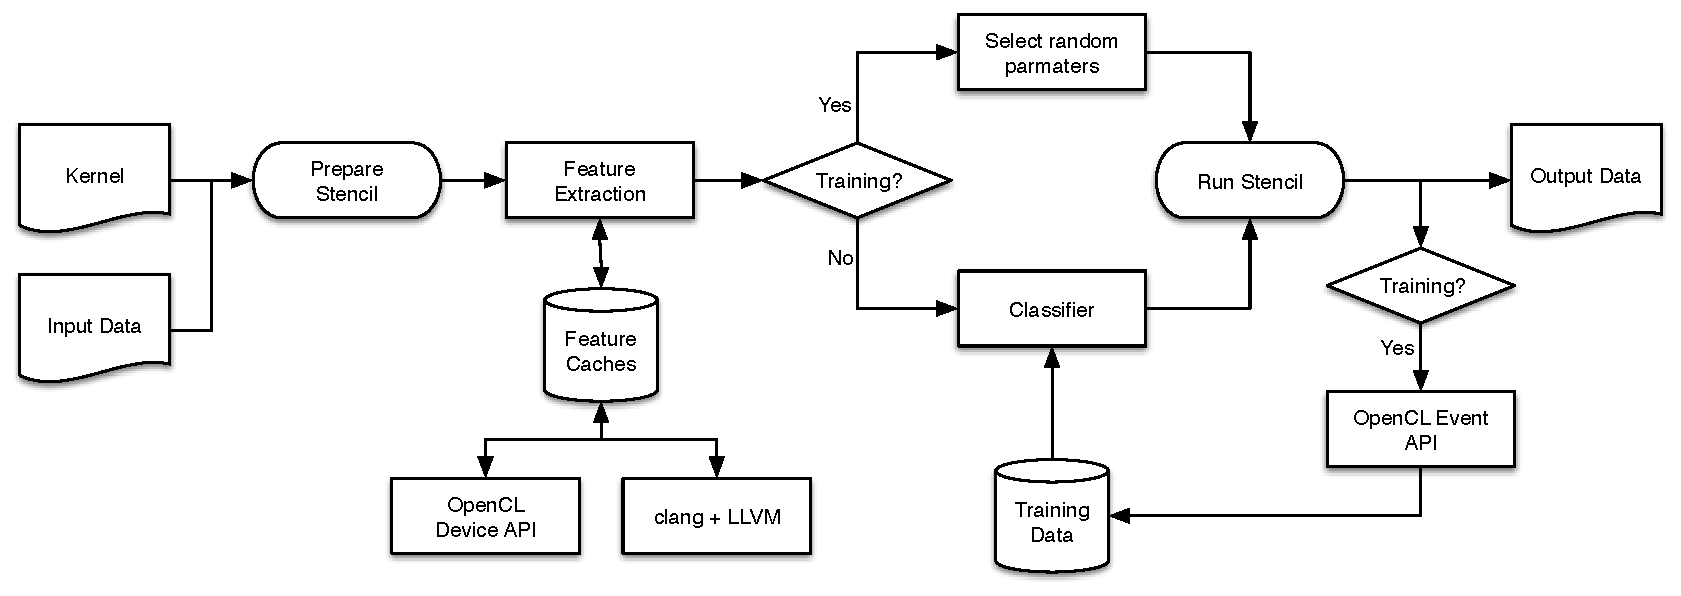
\includegraphics[width=.95\textwidth]{omnitune-system-flow}
\caption{%
  Integration of OmniTune into SkelCL stencil execution.%
}
\label{fig:omnitune-system-flow}
\end{figure}



% \section{Machine Learning and Performance Tuning}
%
% \TODO{We're always dealing with a sparsity in data.}

\section{Collective Tuning and the Client-Server Model}

Omnitune uses a three tier client-server model, illustrated in
Figure~\ref{fig:omnitune-system-overview}. Target applications request
optimisation parameter values from a system-wide server, which in turn
communicates with a global database to add and receive training
data. A set of caches in the system wide server act as a buffer
between the client and the global database to minimise the latency of
requests for optimisation parameter values.

This design has two primary advantages: the first is that it decouples
the autotuning logic from that of the client program, allowing
developers to easily repurpose the autotuning framework to target
additional optimisation parameters through a system of plugins; the
second advantage is that this enables collective tuning, in which
training data gathered from a range of devices can be accessed and
added to by any OmniTune server. Anyone downloading a copy of OmniTune
will instantly have access to the global database of training data,
including the \input{gen/num_samples} runtimes which were collected to
write this thesis.

\FIXME{This last sentence is not currently implemented, since I'm
  using only a system-wide database. I'll need to implement a MySQL
  interface or reword.}

\begin{figure}
\centering
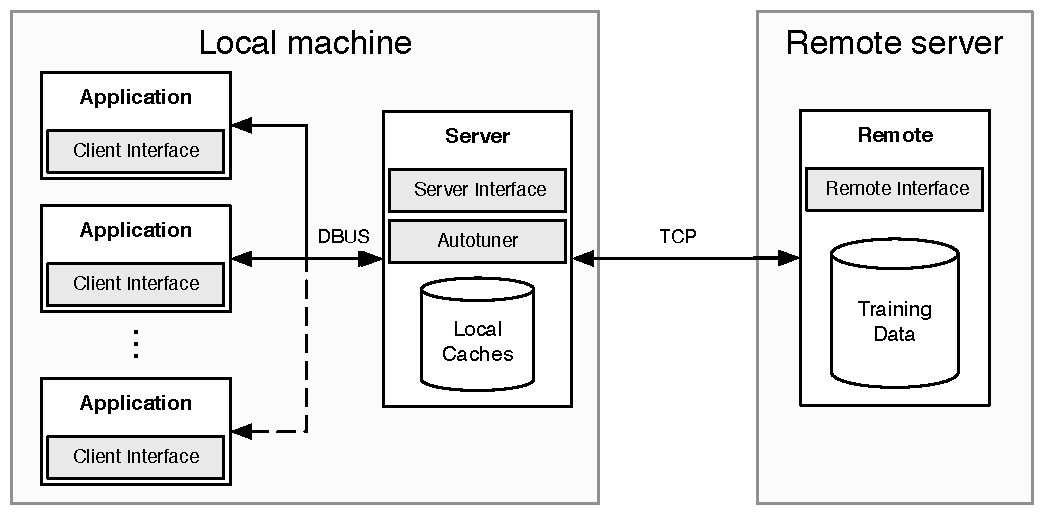
\includegraphics[width=.95\textwidth]{omnitune-system-overview}
\caption{%
  High level system overview of OmniTune.%
}
\label{fig:omnitune-system-overview}
\end{figure}

As discussed in \xref{related work}, common implementations of
autotuning in the literature either: embed the autotuning logic within
the target applications, or take a ``meta-scripting'' approach in
which the autotuner is a standalone program which must be invoked by
the user to tune a target application. The approach taken in this work
aims to capture the advantages of both techniques by implementing an
autotuning service with communication logic embedded in the target
applications. The resulting design consists of three sets of
components: clients, servers, and a global
database. Figure~\ref{fig:omnitune-comms} shows a typical pattern of
communication between the components.

\begin{figure}
\centering
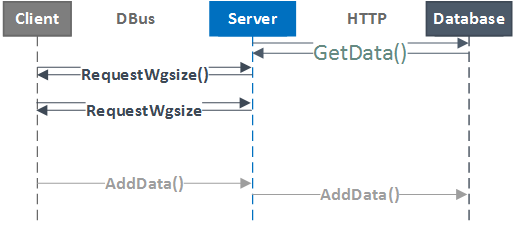
\includegraphics[width=.8\textwidth]{img/omnitune-comms}
\caption{%
  Communication pattern between OmniTune components.%
}
\label{fig:omnitune-comms}
\end{figure}

\TODO{Advantages: asynchronous communication with ``the
  cloud''. Expensive tasks such as model building aren't bound by the
  lifespan of the client application. Lightweight handling of multiple
  connections.}


\subsection{Database: Distributed Training Data}

A master server maintains a common store of all performance
data. \TODO{Write-up schemas, table normal forms, checksum IDs,
  \ldots}


\subsection{Server: Autotuning Engine}

For each autotuning-capable machine, a system-level daemon hosts a
DBus session bus which client processes communicate with. This daemon
acts as an intermediate between the training data and the client
applications, \emph{serving} requests for optimisation parameter
values. The server is implemented as a standalone Python program. On
launch, the server requests the latest training data from the master
database, it then builds the relevant models for performing prediction
of optimisation parameter values. \TODO{Synchronisation, local caching
  and of global DB state.}

OmniTune servers use a plugin system to host proxies that interface
with target applications. Proxies are application-specific, for
example, there is a proxy which implements autotuning of workgroup
size for SkelCL stencils. This proxy exposes two public methods,
\texttt{RequestWgsize} and \texttt{RequestTrainingWgsize}, shown in
Listing~\ref{lst:omnitune-proxy}.

In addition to interfacing with client applications and the database,
OmniTune servers contains a library of generic machine learning tools,
interfacing with Weka\footnote{http://www.cs.waikato.ac.nz/ml/weka/}
using the JNI to perform classification. Each proxy performs feature
extraction of incoming client requests and uses the common machine
learning tools to predict optimal parameter values. \TODO{Plugins
  allow separation of concerns.}

\lstinputlisting[
  language=Python,
  float,
  floatplacement=t,
  label=lst:omnitune-proxy,
  caption={%
    Public OmniTune proxy interface for SkelCL autotuning.%
  }
]{dat/omnitune-skelcl-proxy.py}


\subsection{Client Interface: Lightweight Communication}

By design, the client-server model allows for enabling autotuning with
a low impact on the target applications. As such, the modifications
required to enable OmniTune support within SkelCL were minimal. The
stencil implementation was modified to use an OmniTune client
interface to suggest workgroup sizes, instead of the hardcoded value
which was previously present
(Listing~\ref{lst:skelcl-set-wgsize}). When a SkelCL stencil is
executed, the client interface synchronously calls the
\texttt{RequestWgsize()} method of the OmniTune server, passing as
arguments the required parameters for feature extraction
(Listing~\ref{lst:omnitune-client}). Feature extraction occurs within
the server, which then classifies the extracted features and returns
the suggested workgroup size to the client SkelCL process.

\note{This is a very low latency operation, and the system daemon can
  handle multiple connections from separate SkelCL processes
  simultaneously (although this is an admittedly unlikely use-case
  given that most GPGPU programs expect to be run in isolation).}

\lstinputlisting[
  language=C++,
  float,
  floatplacement=t,
  label=lst:skelcl-set-wgsize,
  caption={
    %
    An extract from the SkelCL stencil implementation, showing the
    call to omnitune client to request workgroup size.
    %
  }
]{dat/skelcl-set-wgsize.cpp}

\lstinputlisting[
  language=C++,
  float,
  floatplacement=t,
  label=lst:omnitune-client,
  caption={
    Implementation of SkeCL's client interface to OmniTune proxy.
  }
]{dat/skelcl-omnitune-client.cpp}


\section{Machine-learning Enabled Autotuning}

The optimisation space presented by selection of workgroup size is
large, complex, and non-linear. In this section I apply the techniques
of machine learning and statistical inference to build a system which
is capable of predicting workgroup sizes for unseen programs, based on
previously collected performance data.


\subsection{Feature Extraction}

As demonstrated in Chapter~\ref{chap:methodology}, the performance of
a workgroup size depends on properties of the architecture, device,
and dataset. The success of a machine learning system depends on the
ability to translate these properties into explanatory variables ---
\emph{features}. For each scenario, a vector of 102 features is
extracted to capture properties of the architecture, device, and
dataset.


\subsubsection{Architectural features}

OmniTune use the OpenCL \texttt{clGetDeviceInfo()} API to query a
number of properties about the target execution device. Examples
include the size of local memory, maximum work group size, number of
compute units, etc.


\subsubsection{Kernel features}

To extract features of the kernel, the user code for the stencil is
passed to the OmniTune server, which compiles the OpenCL kernel to
LLVM IR bitcode. The \texttt{opt} \texttt{InstCount} statistics pass
is used to obtain instruction counts for each type present in the
kernel, and the total number of instructions. The instruction counts
for each type are divided by the total number of instructions to
produce a \emph{ratio} of instruction for that type. Examples include
total static instruction count, ratio of instructions per type, ratio
of basic blocks per instruction, etc.

\TODO{Write an experiment for which static instruction counts fall
  down. For example, two programs with similar instruction counts, one
  with a huge loop, the other with straight line code.}


\subsubsection{Dataset features}

Dataset features are extracted from the SkelCL container type. The
extracted features are the input and output data types, and the 2D
grid size.

See Table~\ref{tab:features} for a full list of features and
types.

\subsubsection{Cost of Feature Extraction}

\TODO{Report feature extraction cost. Note that feature vectors are
  cached so this cost is a one-off, subsequent iterations are just a
  table lookup.}

\begin{table}
\begin{multicols}{2}
\scriptsize
\centering
\rowcolors{2}{white}{gray!25}
\begin{multicols}{2}
\scriptsize
\centering
\rowcolors{2}{white}{gray!25}
\begin{multicols}{2}
\scriptsize
\centering
\rowcolors{2}{white}{gray!25}
\input{gen/tab/features.1}
\vfill
\columnbreak
\rowcolors{2}{white}{gray!25}
\input{gen/tab/features.2}
\end{multicols}

\vfill
\columnbreak
\rowcolors{2}{white}{gray!25}
\begin{multicols}{2}
\scriptsize
\centering
\rowcolors{2}{white}{gray!25}
\input{gen/tab/features.1}
\vfill
\columnbreak
\rowcolors{2}{white}{gray!25}
\input{gen/tab/features.2}
\end{multicols}

\end{multicols}

\vfill
\columnbreak
\rowcolors{2}{white}{gray!25}
\begin{multicols}{2}
\scriptsize
\centering
\rowcolors{2}{white}{gray!25}
\begin{multicols}{2}
\scriptsize
\centering
\rowcolors{2}{white}{gray!25}
\input{gen/tab/features.1}
\vfill
\columnbreak
\rowcolors{2}{white}{gray!25}
\input{gen/tab/features.2}
\end{multicols}

\vfill
\columnbreak
\rowcolors{2}{white}{gray!25}
\begin{multicols}{2}
\scriptsize
\centering
\rowcolors{2}{white}{gray!25}
\input{gen/tab/features.1}
\vfill
\columnbreak
\rowcolors{2}{white}{gray!25}
\input{gen/tab/features.2}
\end{multicols}

\end{multicols}

\end{multicols}

\caption{Feature names and types, describing the dataset, kernel,
  and device.}
\label{tab:features}
\end{table}


\subsection{Predicting Optimal Workgroup Sizes}

The first approach to selecting workgroup sizes is to convert the set
of oracle workgroup sizes into a hypothesis space and then use a
classifier to predict the oracle workgroup size for a given set of
features. To evaluate this approach, a subset of scenarios
$S_{training} \subset S$ are labelled with their oracle workgroup
size. The classifier is trained on this labelled training data, and
tested using a set of unseen scenarios
$S_{testing} = S - S_{training}$. The performance of each predicted
oracle workgroup size is compared against the true oracles for that
set.


\subsubsection{Satisfying Constraints}

The set of workgroup sizes which a classifier may predict is defined
by the oracle workgroup sizes of the training data:

\begin{equation}
W_{training} = \{ \Omega(s) | s \in S_{training} \}
\end{equation}

This does not guarantee that the set of workgroup sizes which may be
predicted is within the set of legal workgroup sizes for each tested
scenario:

\begin{equation}
W_{training} \nsubseteq \cup \{ W_{legal}(s) | s \in S_{testing} \}
\end{equation}

\TODO{2 solutions: satisfy constraint at classification time
  (i.e. error handlers), or at training time (i.e. one classifier per
  max-wg-size)\ldots}

As a result, it is possible that a classifier will predict a workgroup
size that is invalid for a given scenario, $w \not\in W_{legal}(s)$.
For these cases, I evaluate the effective of three fallback strategies
to select a legal workgroup size:

\begin{enumerate}
\item \emph{Baseline} --- select the workgroup size which is known to
  be safe and provides the highest average case performance on
  training data.
\item \emph{Random} --- select a random workgroup size which is known
  to be legal $w \in W_{legal}(s)$.
\item \emph{Reshape} --- scale the predicted workgroup size
  proportionally so that it fits within the space of legal workgroup
  sizes, $w < W_{max}(s)$. This attempts to preserve ``shape'' of the
  predicted workgroup size.
\end{enumerate}

See Algorithm~\ref{alg:autotune-classification} for definitions. The
evaluation compares the average performance achieved using each
fallback strategy, along with the percentage of cases for which these
fallback strategies were required.

\begin{algorithm}
\begin{algorithmic}[1]
\Require kernel features $k$, hardware features $h$, dataset features
$d$.
\Ensure workgroup size $w$

\Procedure{Default}{w, a, k, d}
\Comment Use the best safe param.
\State $w \leftarrow \text{classify}(a, k, d)$
\If{$w \in W_{legal}(s)$}
    \State \textbf{return} $w$
\Else
  \State \textbf{return} $\underset{w \in W_{safe}}{\argmax}
\left(
  \prod_{s \in S_{training}} p(s, w)
\right)^{1/|S_{training}|}$
\EndIf
\EndProcedure
\item[]

\Procedure{Random}{w, a, k, d}
\Comment Use a random param from $W_{legal}$.
\State $w \leftarrow \text{classify}(a, k, d)$
\If{$w \in W_{legal}(s)$}
    \State \textbf{return} $w$
\Else
  \State \textbf{return} random choice $w \in W_{legal}$
\EndIf
\EndProcedure
\item[]

\Procedure{Reshape}{w, a, k, d}
\Comment Coerce params to be legal.
\State $w \leftarrow \text{classify}(a, k, d)$
\If{$w \in W_{legal}(s)$}
    \State \textbf{return} $w$
\Else
  \State $d_{min} \leftarrow \infty$
  \State $w_{closest} \leftarrow \text{null}$
  \For{$c \in W_{legal}$}
    \State $d \leftarrow \sqrt{\left(c_r - w_r\right)^2 + \left(c_c - w_c\right)^2}$
    \If{$d < d_{min}$}
      \State $d_{min} \leftarrow d$
      \State $w_{closest} \leftarrow c$
    \EndIf
  \EndFor
  \State \textbf{return} $w_{closest}$
\EndIf
\EndProcedure
\end{algorithmic}

\caption{Select optimal workgroup size using classification}
\label{alg:autotune-classification}
\end{algorithm}

\TODO{Implement and evaluate classification using one classifier for
  each unique $w \in \cup \{ W_{max}(s) | s \in S_{training} \}$. This
  would be an alternative method of overcoming the invalid prediction
  problem.}

\subsection{Predicting Stencil Code Runtime}

\TODO{The first approach requires very expensive training and isn't
  amenable to online tuning\ldots} A second approach to selecting the
workgroup size is to attempt to directly predict the runtime of a
given workload. Given a regressor $f(a,k,d,w)$ which predicts the
runtime of a program given a set of architecture, kernel, and dataset
features $a,k,d$, and workgroup size $w$, the predicted optimal
workgroup size is the $w$ value which minimises the output of the
regressor:

\begin{equation}
  \underset{w \in W_{legal}(s)}{\argmin} f(a,k,d,w)
\end{equation}

By predicting the runtimes of only the workgroup sizes from within
$W_{legal}(s)$, we overcome the issue of predicting invalid workgroup
sizes. Training a regressor to predict runtimes requires a set of
training data which contains workgroup sizes as an additional feature,
and the measured mean runtime as the label.

% \begin{algorithm}
% \begin{algorithmic}[1]
\Require kernel features $k$, hardware features $h$, dataset features
$d$.
\Ensure predicted oracle workgroup size $\bar{\Omega}(s)$
\State $C \leftarrow \{c_1, c_2, \ldots, c_n \}$
\Comment Set of all workgroup sizes $\le k.\text{max\_wgsize}$
\State \textbf{return} $\underset{c \in C}{\argmin} f(k,h,d,c)$
\end{algorithmic}

% \caption{Selecting workgroup size using runtime regression}
% \label{alg:autotune-runtime-regression}
% \end{algorithm}

\subsection{Predicting Relative Performance}

Accurately predicting the runtime of an arbitrary program is a
difficult problem due to the impacts of flow control. It may be
effective to instead predict the \emph{relative} performance of two
different workgroup sizes for the same program. To do this, we select
a baseline workgroup size $w_b \in W_{safe}$, and train a regressor
$g(a,k,d,w)$ with training data labelled with the relative performance
over the baseline $r(w, w_b)$. Predicting the optimal workgroup
requires maximising the output of the regressor:

\begin{equation}
  \underset{w \in W_{legal}(s)}{\argmax} g(a,k,d,w)
\end{equation}

% \begin{algorithm}
% \begin{algorithmic}[1]
\Require kernel features $k$, hardware features $h$, dataset features
$d$.
\Ensure workgroup size $w$
\State $C \leftarrow \{c_1, c_2, \ldots, c_n \}$
\Comment Set of all workgroup sizes $\le k.\text{max\_wgsize}$
\State \textbf{return} $\underset{c \in C}{\argmax} f(k,h,d,c)$
\end{algorithmic}

% \caption{Selecting workgroup size using speedup regression}
% \label{alg:autotune-speedup-regression}
% \end{algorithm}


\subsection{Meta-tuning: a Hybrid Approach}

\TODO{Implement and test. See Algorithm~\ref{alg:autotune-hybrid}.}

\begin{algorithm}
\begin{algorithmic}[1]
\Require kernel features $k$, hardware features $h$, dataset features $d$.
\Ensure workgroup size $w$

\State $r \leftarrow \underset{w \in W_{legal}(s)}{\min} f(k,h,d,w)$
\Comment Predict minimum runtime.
\State $w \leftarrow \underset{w \in W_{legal}(s)}{\argmin} f(k,h,d,w)$
\Comment Workgroup size for $r$.
\State $t_r \leftarrow$ measure runtime of program with $w$
\If{$t_r \approx r$}
  \State \textbf{return} $w$
\Comment Predicted runtime is accurate.
\Else
   \State $W \leftarrow W_{legal}(s)$
   \State converged $\leftarrow$ false
   \State $w_b \leftarrow$ baseline value
   \State $t_b \leftarrow$ measure runtime of runtime of program with $w_b$
   \While{not converged}
     \State $s \leftarrow \underset{w \in W}{\max} g(k,h,d,w)$
     \Comment Predict best speedup.
     \State $w \leftarrow \underset{w \in W}{\argmax} g(k,h,d,w)$
     \Comment Workgroup size for $s$.
     \State $t \leftarrow$ measure runtime of program with $s$
     \If{$t_b / t \approx s$}
       \State converged = true
       \Comment Predicted speedup is accurate.
     \Else
       \State $W = W - \{w\}$
     \EndIf
   \EndWhile
   \State \textbf{return} $w$
\EndIf
\end{algorithmic}

\caption{Selecting workgroup size using a hybrid approach}
\label{alg:autotune-hybrid}
\end{algorithm}

\section{Summary}

This chapter has described the design and implementation of OmniTune,
a distributed autotuner which is capable of performing runtime
prediction of optimal workgroup sizes for SkelCL stencils using a
variety of machine learning approaches. OmniTune uses a client-server
model to decouple the autotuning logic from target programs and to
maintain separation of concerns. It uses lightweight inter-process
communication to achieve low latency autotuning, and uses caches and
lookup tables to minimise the one-off costs of feature
extraction. \TODO{Summarise ML approaches\ldots}
